\begin{figure}[h!]
  \begin{minipage}[c]{0.45\textwidth}
    \caption{
      \textbf{The smooth approach is expected to be more robust than the bin approach.} Both panels depict the same mutation location data for a hypothetical chromosome, with the black dots below the x-axis representing the true location of mutations. The conventional bin representation counts the number of mutations in each green bin. Shifting the bin boundaries from panel (a) to panel (b) changes the counts. On the contrary, the smooth representation of GLE is depicted by the purple dots on the purple line remains the same.
    } \label{fig:mutdistribution_demo}
  \end{minipage}\hfill
  \begin{minipage}[c]{0.55\textwidth}
    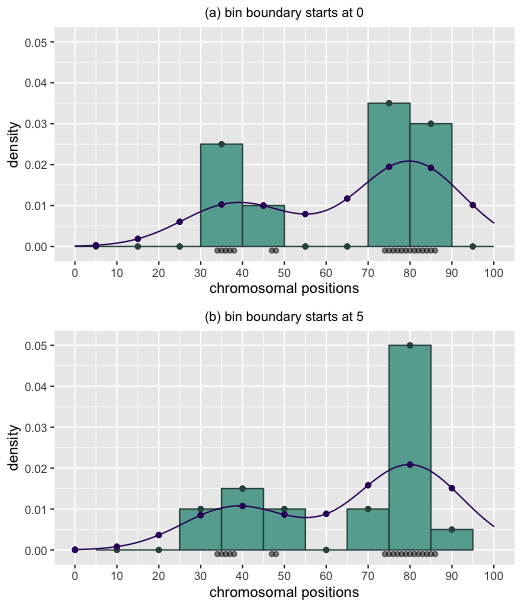
\includegraphics[width=\textwidth]{graphics/mutdistribution_demo.png}
  \end{minipage}
\end{figure}
